\pdfminorversion=4 % for acroread
\documentclass[aspectratio=169,t,xcolor={usenames,dvipsnames}]{beamer}
%\documentclass[t,handout,xcolor={usenames,dvipsnames}]{beamer}
\usepackage{../beamerstyle}
\usepackage{dsfont}
\usepackage{bm}
\usepackage[english]{babel}
\usepackage[utf8]{inputenc}
\usepackage{graphicx}
\usepackage{algorithm}
\usepackage[ruled,vlined,algo2e,linesnumbered]{algorithm2e}
%\usepackage[boxed,vlined]{algorithm2e}
\usepackage{hyperref}
\usepackage{booktabs}
\usepackage{mathtools}

\usepackage{amsmath,amssymb}
\usepackage{listings}
\lstset{frame=lines,framesep=3pt,numbers=left,numberblanklines=false,basicstyle=\ttfamily\small}

\usepackage{subfig}
\usepackage{multicol}
%\usepackage{appendixnumberbeamer}
%
\usepackage{tcolorbox}

\usepackage{pgfplots}
\usepackage{tikz}
\usetikzlibrary{trees} 
\usetikzlibrary{shapes.geometric}
\usetikzlibrary{positioning,shapes,shadows,arrows,calc,mindmap}
\usetikzlibrary{positioning,fadings,through}
\usetikzlibrary{decorations.pathreplacing}
\usetikzlibrary{intersections}
\usetikzlibrary{positioning,fit,calc,shadows,backgrounds}
\pgfdeclarelayer{background}
\pgfdeclarelayer{foreground}
\pgfsetlayers{background,main,foreground}
\tikzstyle{activity}=[rectangle, draw=black, rounded corners, text centered, text width=8em]
\tikzstyle{data}=[rectangle, draw=black, text centered, text width=8em]
\tikzstyle{myarrow}=[->, thick, draw=black]

% Define the layers to draw the diagram
\pgfdeclarelayer{background}
\pgfdeclarelayer{foreground}
\pgfsetlayers{background,main,foreground}

%\usepackage{listings}
%\lstset{numbers=left,
%  showstringspaces=false,
%  frame={tb},
%  captionpos=b,
%  lineskip=0pt,
%  basicstyle=\ttfamily,
%%  extendedchars=true,
%  stepnumber=1,
%  numberstyle=\small,
%  xleftmargin=1em,
%  breaklines
%}

 
\definecolor{blue}{RGB}{0, 74, 153}

\usetheme{Boadilla}
%\useinnertheme{rectangles}
\usecolortheme{whale}
\setbeamercolor{alerted text}{fg=blue}
\useoutertheme{infolines}
\setbeamertemplate{navigation symbols}{\vspace{-5pt}} % to lower the logo
\setbeamercolor{date in head/foot}{bg=blue} % blue
\setbeamercolor{date in head/foot}{fg=white}
\setbeamercolor{author in head/foot}{bg=blue} %blue
\setbeamercolor{title in head/foot}{bg=blue} % blue
\setbeamercolor{title}{fg=white, bg=blue}
\setbeamercolor{block title}{fg=white,bg=blue}
\setbeamercolor{block body}{bg=blue!10}
\setbeamercolor{frametitle}{fg=white, bg=blue}
\setbeamercovered{invisible}

\makeatletter
\setbeamertemplate{footline}
{
  \leavevmode%
  \hbox{%
  \begin{beamercolorbox}[wd=.333333\paperwidth,ht=2.25ex,dp=1ex,center]{author in head/foot}%
    \usebeamerfont{author in head/foot}\insertshortauthor
  \end{beamercolorbox}%
  \begin{beamercolorbox}[wd=.333333\paperwidth,ht=2.25ex,dp=1ex,center]{title in head/foot}%
    \usebeamerfont{title in head/foot}\insertshorttitle
  \end{beamercolorbox}%
  \begin{beamercolorbox}[wd=.333333\paperwidth,ht=2.25ex,dp=1ex,right]{date in head/foot}%
    \usebeamerfont{date in head/foot}Week \@week, Topic \@topicnumber, Slide \insertframenumber{}\hspace*{2em}
%    \insertframenumber\hspace*{2ex} 
  \end{beamercolorbox}}%
  \vskip0pt%
}

\newcommand{\@week}{0}
\newcommand{\@topicnumber}{0}
\newcommand{\week}[1]{\renewcommand{\@week}{#1}}
\newcommand{\topicnumber}[1]{\renewcommand{\@topicnumber}{#1}}

\makeatother

%\pgfdeclareimage[height=1.2cm]{automl}{images/logos/automl.png}
%\pgfdeclareimage[height=1.2cm]{freiburg}{images/logos/freiburg}

%\logo{\pgfuseimage{freiburg}}

\input{../latex_main/macros}




\newcommand{\inducer}{\mathcal{I}}
\newcommand{\R}{\mathds{R}}

%The following might look confusing but allows us to switch the notation of the optimization problem independently from the notation of the hyper parameter optimization
\newcommand{\xx}{\conf} %x of the optimizer
\newcommand{\xxi}[1][i]{\conf_{#1}} %i-th component of xx (not confuse with i-th individual)
\newcommand{\XX}{\pcs} %search space / domain of f
\newcommand{\f}{\cost} %objective function

\newenvironment{blocki}[1] % itemize block
{
 \begin{block}{#1}\begin{itemize}
}
{
\end{itemize}\end{block}
}

\title[AutoML: Hyperparameter Optimization]{AutoML: Hyperparameter Optimization}
%\subtitle{Overview for this Week} %To be defined in source!
%TODO: change authors!
\author[Jakob Richter]{Bernd Bischl \and Frank Hutter \and Lars Kotthoff\newline \and Marius Lindauer}
\institute{}
\date{}


\usepackage[normalem]{ulem}
\usepackage{pifont}
\usepackage{relsize}
\renewcommand{\lit}[1]{{\smaller\color{black!60}[#1]}}
\title[AutoML: Practical]{AutoML: Practical Considerations}
\subtitle{Machine Learning Pipelines}
\author[Janek Thomas]{Bernd Bischl \and Frank Hutter \and Lars Kotthoff\newline \and Marius Lindauer \and \underline{Janek Thomas} \and Joaquin Vanschoren}


\begin{document}
	
	\maketitle
	
    \begin{frame}{Pipelines and Workflows}
		
		% Most preprocessing steps have parameters or can be switched on/off in the pipeline.
		
		% \vspace{1em}
		
		% \textbf{Goal:} Find optimal preprocessing parameters $\rightarrow$ HPO
		
		To build AutoML systems we need a language to describe: 

		\begin{itemize}
			\item Machine learning algorithms
			\item Preprocessing operations
			\item Ensemble methodes like model averaging and stacking
			\item How data is passed from one stage to another
		\end{itemize}

		\begin{center}
		\includegraphics[page=7, width=0.7\textwidth, trim=200 0 30 190, clip]{images/mlr3Pipelines_graphics}
		\end{center}

	\end{frame}

	\begin{frame}{Pipelines and Workflows}
		\begin{columns}
			\begin{column}{0.5\textwidth}
				\textbf{Nodes:} What is happening? 
				\begin{center}
					\includegraphics[page=8, width=\textwidth, trim=200 0 30 190, clip]{images/mlr3Pipelines_graphics}
				\end{center}
			\end{column}%
			\begin{column}{0.5\textwidth}
				\textbf{Edges:} In what sequence is it happening? 
				\begin{center}
					\includegraphics[page=9, width=\textwidth, trim=200 0 30 190, clip]{images/mlr3Pipelines_graphics}
				\end{center}
			\end{column}
		\end{columns}
		
	\vspace{1cm}

	$\longrightarrow$ We represent a ML workflow as a stateful directed acyclical graph with nodes of operations and edged of data flow between them.

	\end{frame}

\begin{frame}{Training nodes}

	Each node can have \textit{hyperparameters} $\pcs_{\text{node}}$, has to be \textit{trained} and can \textit{predict}.

	\begin{center}
		\includegraphics[page=2, width=0.6\textwidth, trim=111 0 130 160, clip]{images/mlr3Pipelines_graphics}
	\end{center}

	Transformed data can be 
	\begin{itemize}
		\item a transformed version of the train/test data for preprocessing nodes, or
		\item predictions for learner nodes.
	\end{itemize}

\end{frame}

\begin{frame}{Linear Pipelines}

A linear pipeline behaves just as a machine learning algorithm.

	\begin{itemize}
		\item Can be evaluated with resampling and ensures that preprocessing does not cause data leakage.
		\item Hyperparameters $\pcs = \pcs_{\text{preproc}} \times \pcs_\inducer$ can be optimized jointly.
	\end{itemize}

	\begin{center}
	\includegraphics[page=19, width=0.7\textwidth, trim=20 60 30 35, clip]{images/mlr3Pipelines_graphics}
	\end{center}
\end{frame}

\begin{frame}{Nodes with Multiple Inputs or Outputs}
	Nodes are not restricted to single inputs and single outputs.
	\begin{center}
		\includegraphics[page=6, width=0.8\textwidth, trim=130 0 100 160, clip]{images/mlr3Pipelines_graphics}
	\end{center}
\end{frame}


\begin{frame}{Ensemble Algorithms}

	This view allows easy representation of different ensemble algorithms:

	\vspace{1cm}

		\begin{columns}
			\begin{column}{0.5\textwidth}
				Bagging:
				\begin{center}
					\includegraphics[page=20, width=\textwidth, trim=0 80 120 85, clip]{images/mlr3Pipelines_graphics}
				\end{center}
			\end{column}
			\begin{column}{0.5\textwidth}
				Stacking:
				\begin{center}
					\includegraphics[page=21, width=\textwidth, trim=0 80 120 85, clip]{images/mlr3Pipelines_graphics}
				\end{center}
			\end{column}
		\end{columns}


\end{frame}

\begin{frame}{Branching}

	To represent the search space of an AutoML system there needs to be a branching node with a selection hyperparameter $\lambda_\text{branch} = (choice_1, ..., choice_k)$.

	\begin{center}
		\includegraphics[page=22, width=0.8\textwidth, trim=40 120 120 80, clip]{images/mlr3Pipelines_graphics}
	\end{center}

\end{frame}


%\item Applying preprocessing to the whole dataset leads to data leakage
%\item Preprocessing should have train and predict steps, too
%\item Can add it to learner, and embed it in CV    
%\item Note: Preprocessing has hyperparameters 
%\item Optimize pipeline jointly: $\pcs = \pcs_{\text{preproc}} \times \pcs_\inducer$ 
%\item Still HPO, not much different than for single learner
%\item $\pcs$ "simply" of higher dimension

	
	\begin{frame}{Example of a simple AutoML system}
	
		\begin{center}
			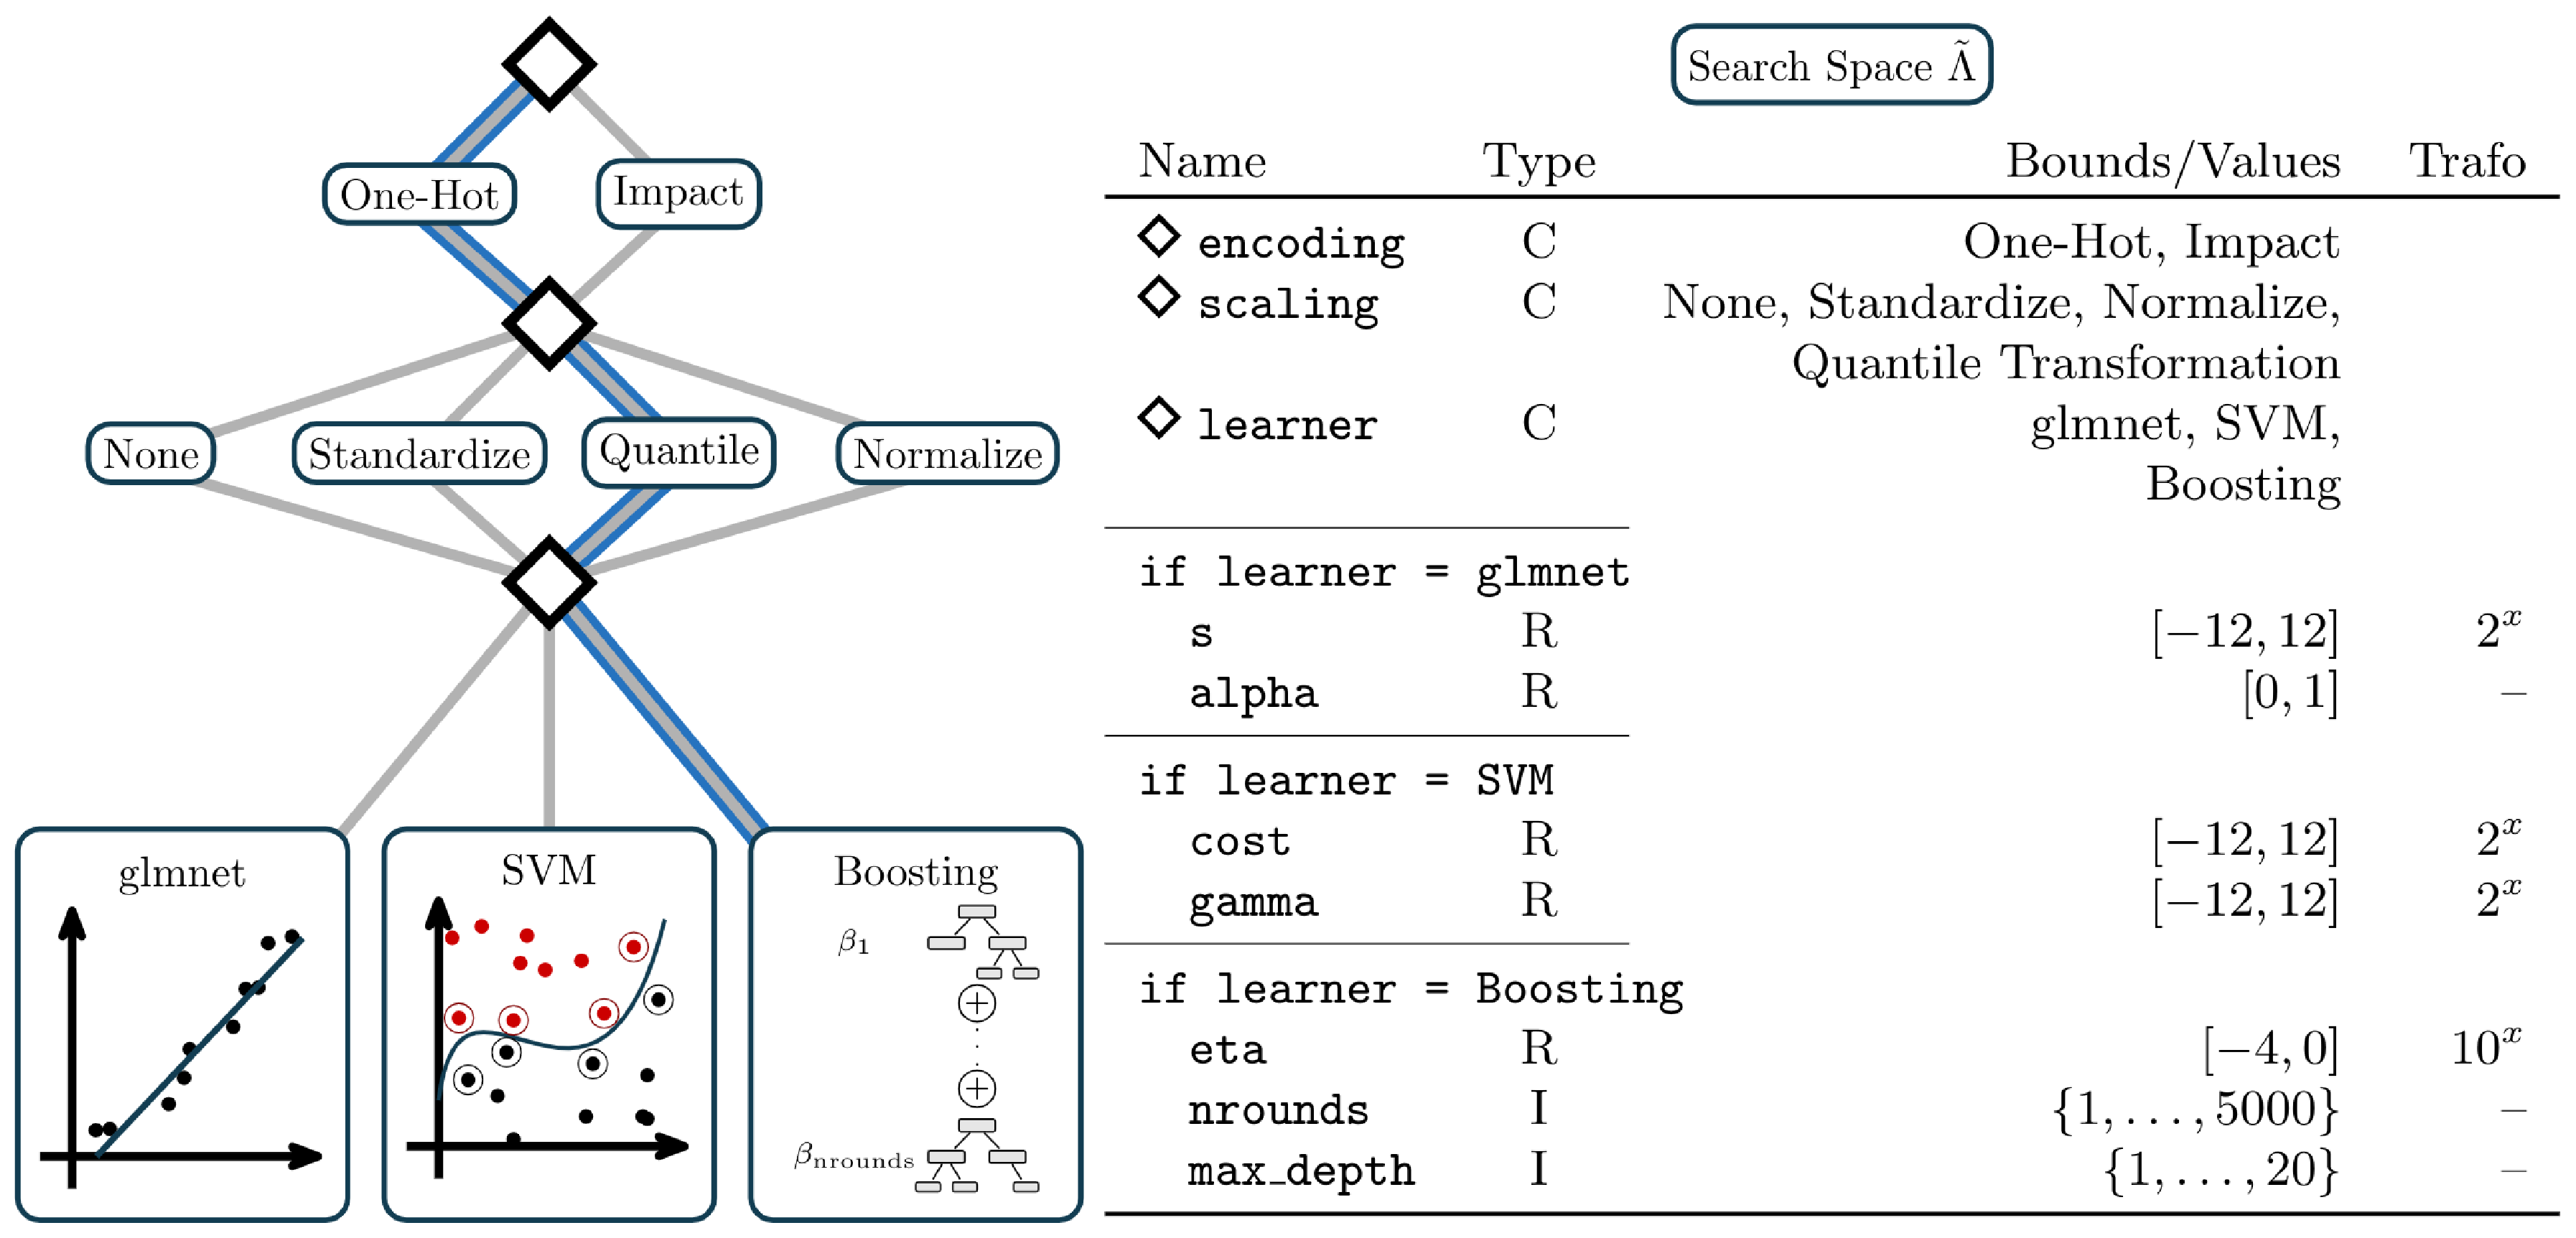
\includegraphics[width = \textwidth]{images/pipeline_with_param_table.eps}
		\end{center}

	\end{frame}
	
	\begin{frame}{Pipeline Systems for Machine Learning Frameworks}

		Different frameworks to define and control such pipelines exist for most common programming languages:

		\begin{itemize}
			\item \texttt{scikit-learn} with \texttt{Pipeline}, \texttt{FeatureUnion} and \texttt{ColumnTransformer} classes for python.
			\item \texttt{mlr3} with \texttt{mlr3pipelines} extension for R.
			\item \texttt{ML.Net} for C\#.
			\item \texttt{tfx} for tensorflow.
			\item \texttt{AutoMLPipeline} for Julia.
			\item ...
		\end{itemize}

	Each framework has slightly different features and limitations. 
	
	\end{frame}

	% \begin{frame}[containsverbatim,allowframebreaks]{Software}
	
	% \begin{itemize}
	%   \item DataRobot (comercial, gui)
	%   \item H20.ai (comercial but open source, r, python)
	%   \item TPOT, Tree-based Pipeline Optimization Tool  (2016-cont, open source, evolutionary approach) % show plot https://github.com/EpistasisLab/tpot
	%   \item AutoWEKA (2016, open source)
	%   \item mlr3automl (2020, prelim)
	%   \item Hyperopt-Sklearn (2014-cont) Only HPO
	%   \item Auto-Sklearn (2.0) (2015-cont) BO, ensembles, meta-learning
	% \end{itemize}
	
	% \end{frame}
	
	
	
\end{document}
